\section{Installation}
This section summarizes the necessary steps to install \MBSim{}.
%
\subsection{Where to find the source code}
The source code of \MBSim{} together with some examples, the necessary \FMatVec{} library, a \HDF{} wrapper for output and the visualisation program \OpenMBV{} can be found at \url{https://github.com} using git\footnote{GIT CHEAT SHEET: \url{https://training.github.com/kit/downloads/github-git-cheat-sheet.pdf}}. Everything is placed under \href{http://www.gnu.org/licenses/lgpl.html}{LGPL}\footnote{see file~\texttt{COPYING} in the root directory of the specific source code}.\par
%
\subsection{Installation procedures}
For the installation of the specific projects always the same \emph{procedures} have to be applied. They are summarized in the following.

\subsubsection{Installation}
\begin{itemize}
	\item \textsc{automake}:
	\begin{itemize}
		\item[] \begin{verbatim}autoreconf -fi\end{verbatim}
	\end{itemize}
	\item \textsc{configure}: 
	\begin{itemize}
		\item[] \begin{verbatim}./configure \end{verbatim}
    \item[] with defining a location for the installation 
                \begin{verbatim}--prefix=$HOME/.../Install\end{verbatim}
		\item[] possibly with project depending FLAGS which we find invoking \begin{verbatim}--help\end{verbatim} 
	\end{itemize}
	\item \textsc{install}
	\begin{itemize}	
		\item \begin{verbatim}make\end{verbatim}
		\item \begin{verbatim}make install\end{verbatim}
	\end{itemize}
\end{itemize}
All procedures belong to the GNU-Build-System (cf.~Sec.~\ref{sec:gnu}).

\subsubsection{Reinstallation/update}
The procedure \textsc{reinstall}
\begin{verbatim}
 make uninstall 
 make clean
 ./config.status --recheck
 make install
\end{verbatim}
newly installs a project with the same configure options used at the previous installation. These information are stored in the file config.status.\\ 
%
The procedure \textsc{update} is similar to the reinstallation:
\begin{verbatim}
 make uninstall 
 make clean
 git pull
 ./config.status --recheck
 make install
\end{verbatim}
For restoring a not-configured version of the project
\begin{verbatim}
 make maintainer-clean
\end{verbatim}
is used. After that \textsc{configure} has to be invoked.

\subsubsection{Uninstallation}
For uninstalling
\begin{verbatim}
 make uninstall
 make clean
\end{verbatim}
has to be called in all directories. If the files created by configure should be deleted, we type 
\begin{verbatim} 
 make distclean 
\end{verbatim} 
%
\begin{figure}[hbt]%
	\centering
    \footnotesize
    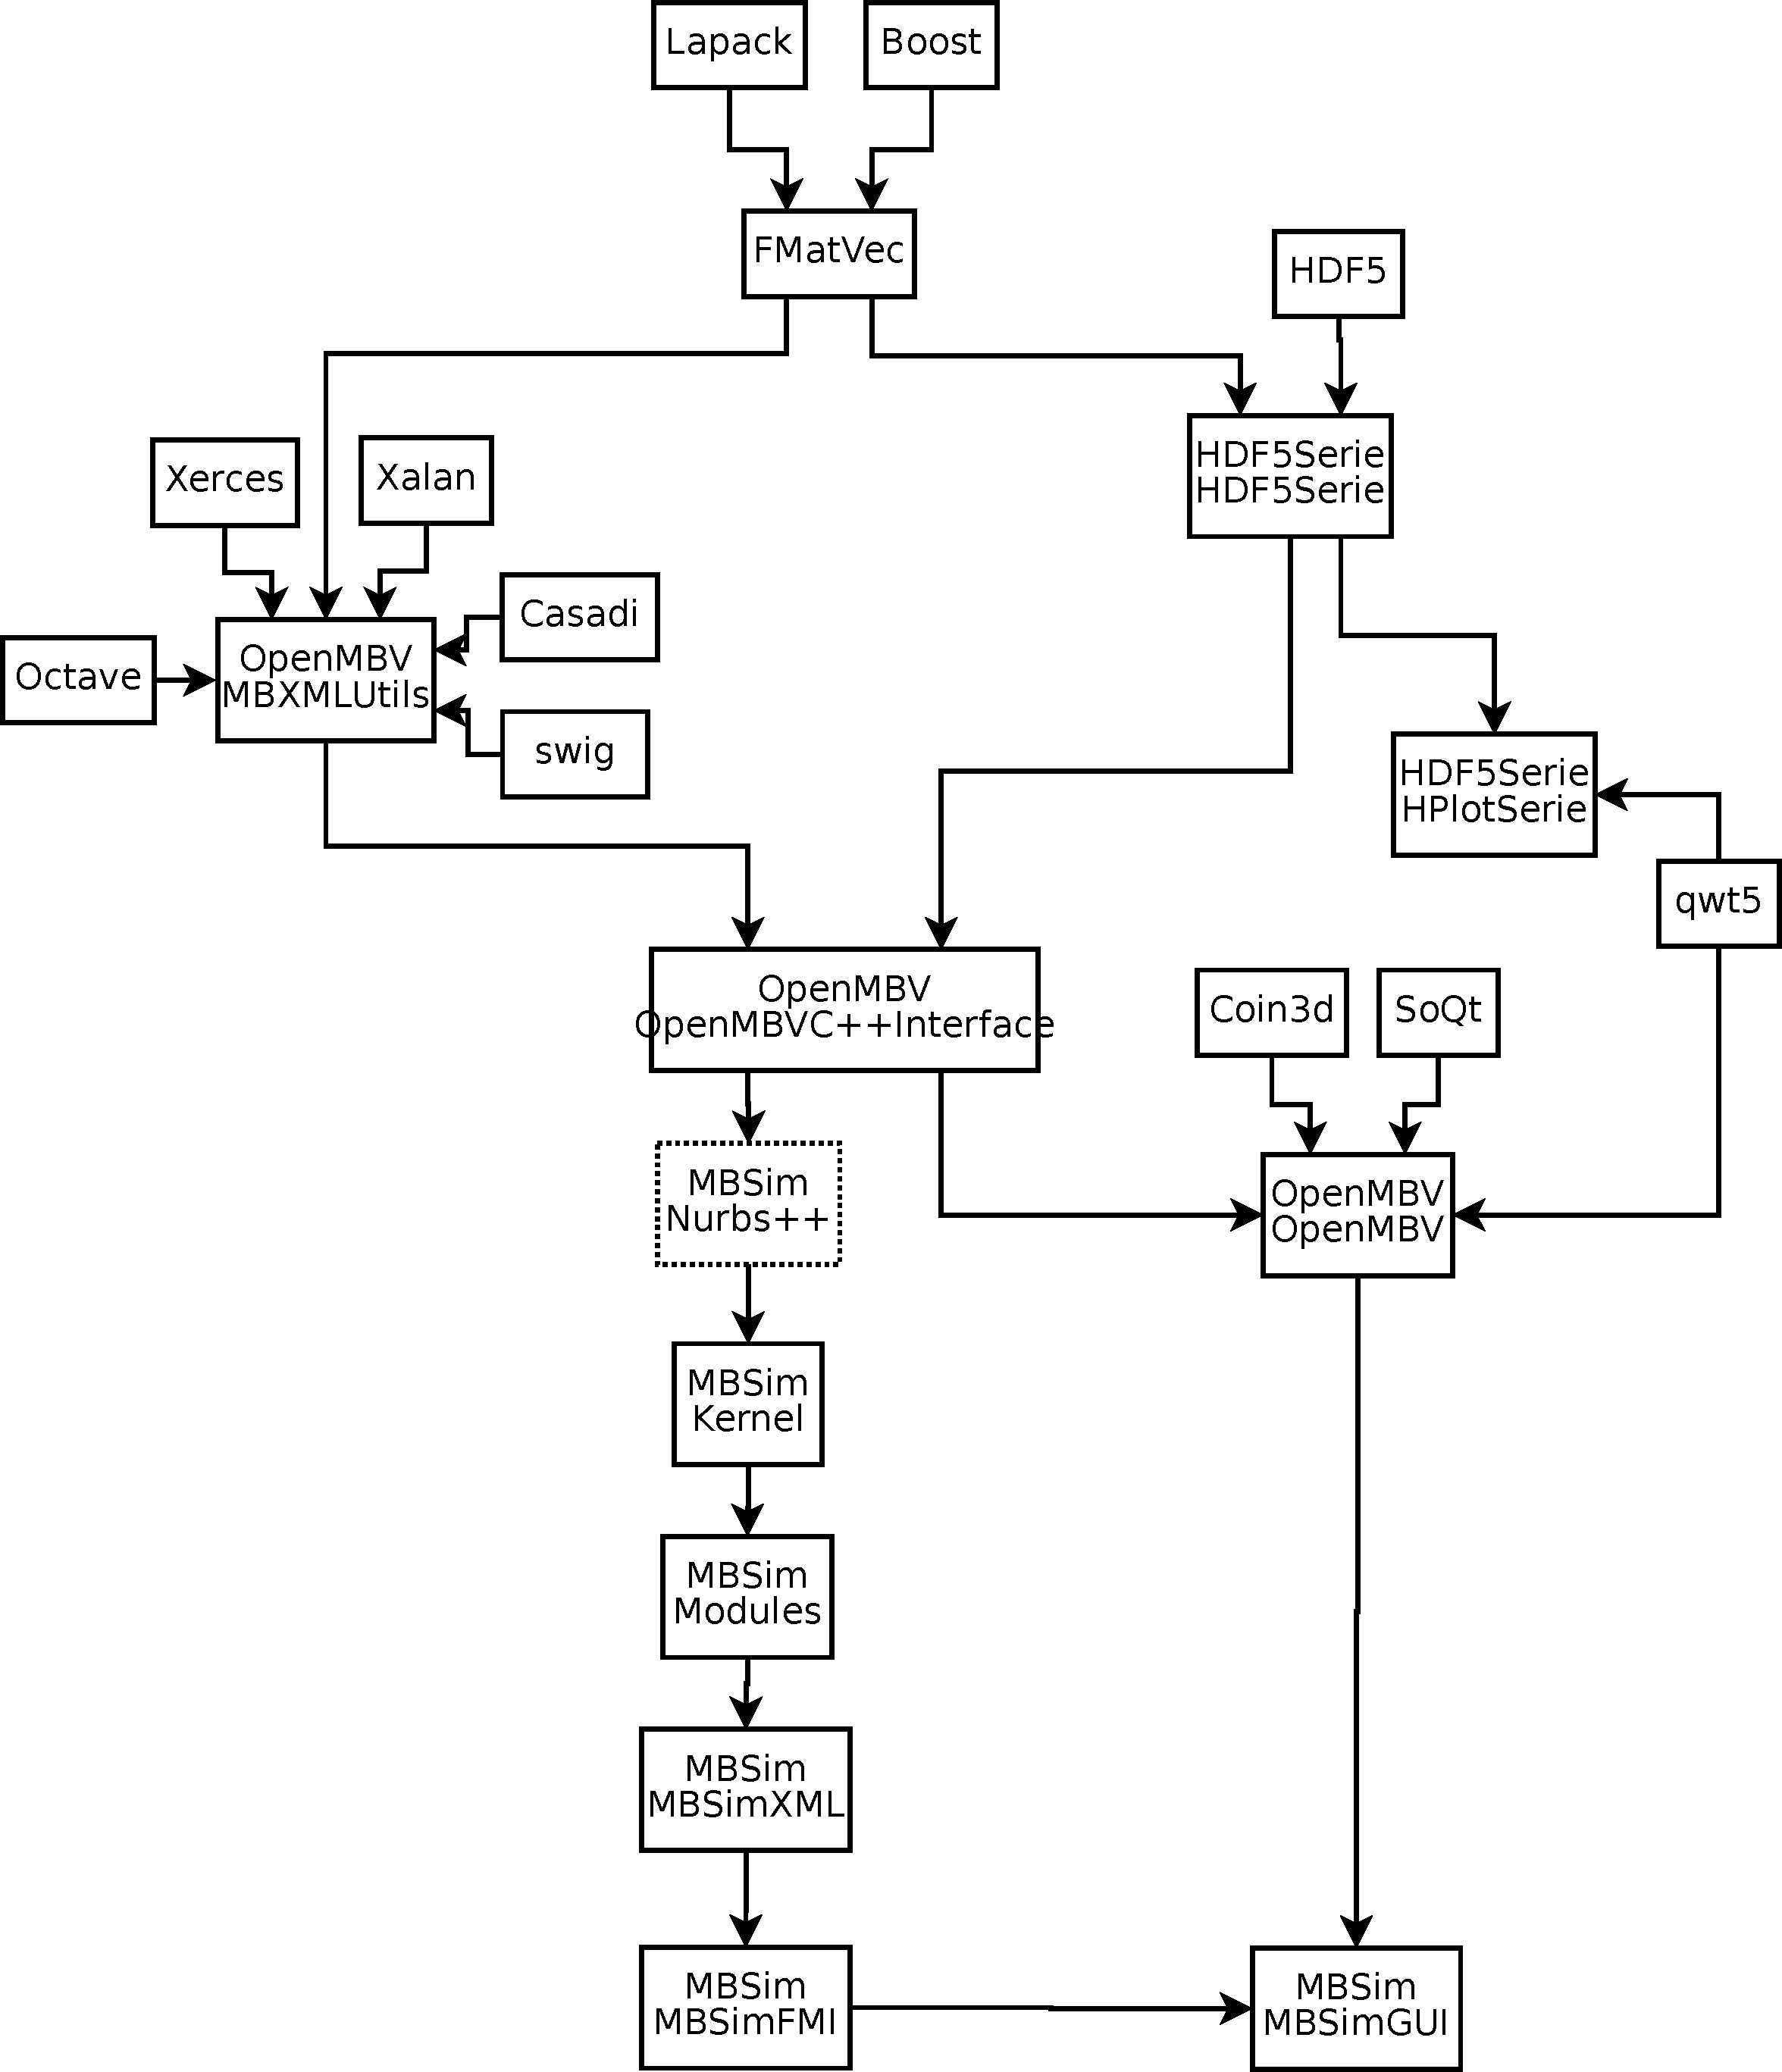
\includegraphics[width=0.95\hsize]{Figures/mbsim_install_flow.pdf}
    \caption{Installation flow for \MBSim{}}
    \label{fig:departure:mbsim:install_flow}
\end{figure}
%
\cleardoublepage
%
\subsection{Installation of the simulation framework\label{sec:install:simulation}}
It is assumed that a directory~\texttt{MBSim} and a directory \texttt{MBSim/Install} have been created in the \texttt{\$HOME} path of the Linux operating system. All projects depend on PKG package administration. The file \texttt{\$HOME/.bashrc} has to be extended with
\begin{verbatim}
 export PKG_CONFIG_PATH=
        "$HOME/MBSim/Install/lib/pkgconfig/:$PKG_CONFIG_PATH"
 export LD_LIBRARY_PATH=
        "$HOME/MBSim/Install/lib/:$LD_LIBRARY_PATH"
\end{verbatim}

\subsubsection{\FMatVec{}}
It is assumed that boost is installed. For the installation the following instructions have to be completed:
\begin{verbatim}
 cd $HOME/MBSim
 git clone https://github.com/mbsim-env/fmatvec.git
 cd $HOME/MBSim/fmatvec
\end{verbatim}
Continue with the procedure \textsc{automake}.
\begin{verbatim}
  mkdir build, cd build
\end{verbatim}
The procedure \textsc{configure} for dynamic compilation is used with
\begin{verbatim}
--prefix=$HOME/MBSim/Install
\end{verbatim}
The code can be compiled and installed with a Doxygen HTML class documentation by \texttt{make doc} and the procedure \textsc{install}.

\subsubsection{\HDFSerie}
%
\paragraph{\HDF}
\HDF{} is a hierarchical data format enabling the effective administration of plot and visualisation data. It can be downloaded as \textbf{source code} ("ALL Platforms") from \url{http://www.hdfgroup.org/HDF5/}, e.g. with version 1.8.15.\\
%
Change to \texttt{\$HOME/MBSim/hdf5}.\\
%
Use the procedure \textsc{configure} for dynamic compilation with
\begin{verbatim}
--prefix=$HOME/MBSim/Install
\end{verbatim}
and the additional FLAG
\begin{verbatim}
 --enable-cxx
\end{verbatim}
Compilation is done with the procedure \textsc{install}.
%
\paragraph{\HDFSerie}
It is assumed that \FMatVec{} is installed. \HDFSerie is available by
\begin{verbatim}
 cd $HOME/MBSim
 git clone https://github.com/mbsim-env/hdf5serie.git
\end{verbatim}
For having \MBSim{} creating \HDF{} files invoke
\begin{verbatim}
 cd $HOME/MBSim/HDF5Serie/hdf5serie
\end{verbatim}
as well as the procedure \textsc{automake}.
\begin{verbatim}
  mkdir build, cd build
\end{verbatim}
Continue with \textsc{configure} for dynamic compilation with
\begin{verbatim}
--prefix=$HOME/MBSim/Install
\end{verbatim}
\texttt{make doc} and \textsc{install} for installation and creation of a Doxygen HTML class documentation.\\
%
Last, \texttt{.bashrc} can be extended with
\begin{verbatim}
alias h5lsserie="$HOME/MBSim/Install/bin/h5lsserie"
alias h5dumpserie="$HOME/MBSim/Install/bin/h5dumpserie"
\end{verbatim}
to gain overall access to the commands \texttt{h5lsserie} and \texttt{h5dumpserie}.

\subsubsection{\OpenMBV{}}
The installation for the simulation framework consists of three steps: first Casadi and the XMLUtils have to be installed, then \MBSim{} needs \textsf{OpenMBV-C++Interface} to create standard data for \OpenMBV{} using C++ programs. The source code is available by
\begin{verbatim}
 cd $HOME/MBSim
 git clone https://github.com/mbsim-env/openmbv.git
\end{verbatim}
%
\paragraph{Casadi}
For installing Casadi, take
\begin{verbatim}
  git clone https://github.com/casadi/casadi.git
\end{verbatim}
create a build-directory
\begin{verbatim}
  cd casadi, mkdir build, cd build
\end{verbatim}
and invoke
\begin{verbatim}
  cmake -DCMAKE_INSTALL_PREFIX=$HOME/MBSim/Install ..
\end{verbatim}
Proceed with
\begin{verbatim}
  make install
\end{verbatim}
%
\paragraph{XMLUtils}
It is assumed that \FMatVec{}, Octave, swig, Xerces, Xalan and Casadi are installed.
\begin{verbatim}
 cd $HOME/MBSim/OpenMBV/mbxmlutils
\end{verbatim} 
and use the procedure \textsc{automake}.
\begin{verbatim}
  mkdir build, cd build
\end{verbatim}
Continue with \textsc{configure} for dynamic compilation with
\begin{verbatim}
--prefix=$HOME/MBSim/Install
\end{verbatim}
and \textsc{install} for installation of an independent XML preprocessor to parse and validate hierarchical XML-files.

\paragraph{OpenMBV-C++Interface}
It is assumed that \HDFSerie{} and XMLUtils are installed. Invoke
\begin{verbatim}
 cd $HOME/MBSim/OpenMBV/openmbvcppinterface
\end{verbatim} 
and the procedure \textsc{automake}.
\begin{verbatim}
  mkdir build, cd build
\end{verbatim}
Continue with \textsc{configure} for dynamic compilation with
\begin{verbatim}
--prefix=$HOME/MBSim/Install
\end{verbatim}
Sometimes trouble with linking \emph{swig} occurs; in this case just set
\begin{verbatim}
--with-swigpath=/nope
\end{verbatim}
to some value such that \emph{swig} is not found on your system.\\
%
\texttt{make doc} and \textsc{install} for installation and creation of a Doxygen HTML class documentation. 
%
\subsubsection{\MBSim}
Necessary for the installation of \MBSim{} is OpenMBV-C++-Interface. For installation, one types
\begin{verbatim}
 cd $HOME/MBSim
 git clone https://github.com/mbsim-env/mbsim.git
\end{verbatim}
%
\paragraph{NURBS thirdparty package}
If you like, you can install the NURBS thirdparty package first, which is necessary for some examples. Invoke the procedure \textsc{automake}.
\begin{verbatim}
  mkdir build, cd build
\end{verbatim}
Continue with \textsc{configure} for dynamic compilation with the prefix
\begin{verbatim}
--prefix=$HOME/MBSim/Install
\end{verbatim}
in \texttt{\$HOME/MBSim/mbsim/thirdparty/nurbs++}.
%
\paragraph{MBSim kernel}
Then proceed and invoke the procedure \textsc{automake}.
\begin{verbatim}
  mkdir build, cd build
\end{verbatim}
Continue with \textsc{configure} for dynamic compilation with
\begin{verbatim}
--prefix=$HOME/MBSim/Install
\end{verbatim}
in \texttt{\$HOME/MBSim/mbsim/kernel}.\\
%
\texttt{make doc} and \textsc{install} to install the basic module and to create a Doxygen HTML class documentation. In
\begin{verbatim}
$HOME/MBSim/mbsim/kernel/xmldoc
\end{verbatim}
invoke \textsc{install} for an XML documentation in\\
\texttt{\$HOME/MBSim/Install/share/mbxmlutils/doc}.
%
\paragraph{Modules}
The following modules are available in MBSim:
%
\begin{itemize}
  \item mbsimControl
  \item mbsimHydraulics
  \item mbsimFlexibleBody
  \item mbsimElectronics
  \item mbsimPowerTrain
  \item mbsimInterface
\end{itemize}
%
The installation proceeds as follows:
\begin{verbatim}
  cd $HOME/MBSim/mbsim/modules/mbsimControl
\end{verbatim}
Invoke the procedure \textsc{automake}.
\begin{verbatim}
  mkdir build, cd build
\end{verbatim}
Continue with \textsc{configure} for dynamic compilation with
\begin{verbatim}
--prefix=$HOME/MBSim/Install
\end{verbatim}
\texttt{make doc} and \textsc{install} to install the signal processing and control module and to create a Doxygen HTML class documentation. In 
\begin{verbatim}
  $HOME/MBSim/mbsim/modules/mbsimControl/xmldoc
\end{verbatim}
invoke \textsc{install} for an XML documentation in\\
\texttt{\$HOME/MBSim/Install/share/mbxmlutils/doc}.\\
%
Proceed in the same way for the other modules in the order as given above.
%
\paragraph{MBSimXML}
MBSimXML offers the possibility to define mechanical systems with XML.
\begin{verbatim}
  cd $HOME/MBSim/mbsim/mbsimxml
\end{verbatim}
Invoke the procedure \textsc{automake}.
\begin{verbatim}
  mkdir build, cd build
\end{verbatim}
Continue with \textsc{configure} for dynamic compilation with
\begin{verbatim}
  --prefix=$HOME/MBSim/Install
\end{verbatim}
and \textsc{install} to install the XML module which contains an executable to invoke the preprocessor. In
\begin{verbatim}
  $HOME/MBSim/mbsim/mbsimxml/xmldoc
\end{verbatim}
invoke \textsc{install} for an XML documentation in\\
\texttt{\$HOME/MBSim/Install/share/mbxmlutils/doc}.
%
\paragraph{MBSimFMI}
MBSimFMI gives an interface for model export. Proceed as follows:
\begin{verbatim}
  cd $HOME/MBSim/mbsim/mbsimfmi
\end{verbatim}
Invoke the procedure \textsc{automake}.
\begin{verbatim}
  mkdir build, cd build
\end{verbatim}
Continue with \textsc{configure} for dynamic compilation with
\begin{verbatim}
  --prefix=$HOME/MBSim/Install
\end{verbatim}
and \textsc{install}.
%
\paragraph{MBSimGUI}
MBSimGUI offers a GUI for \MBSim{}. If we have installed \OpenMBV{}, we can install it.
\begin{verbatim}
  cd $HOME/MBSim/mbsim/mbsimgui
\end{verbatim}
Invoke the procedure \textsc{automake}.
\begin{verbatim}
  mkdir build, cd build
\end{verbatim}
Continue with \textsc{configure} for dynamic compilation with
\begin{verbatim}
  --prefix=$HOME/MBSim/Install
\end{verbatim}
and \textsc{install}.

\subsubsection{Examples}
The examples are used for testing successful installation. There are two possibilities:
\begin{enumerate}
\item Change to the specific directory \texttt{\$HOME/MBSim/mbsim/examples/*} and type \texttt{make} to create an executable. The simulation starts with the command~\texttt{./main}. The results are visualised with the command~\texttt{openmbv} and plotted with~\texttt{h5plotserie} after having installed the visualisation framework (Sec.~\ref{sec:install:visualisation} and \ref{sec:plot}).
\item Use the script \texttt{python runexamples.py} in \texttt{\$HOME/MBSim/mbsim/examples} to compile, run and test each example. See \texttt{python runexamples.py --help} for additional information.
\end{enumerate}
%
\subsection{Installation of the visualisation framework\label{sec:install:visualisation}}
It is assumed, that a directory~\texttt{OpenMBV} and a directory \texttt{OpenMBV/Install} has been created in the \texttt{\$HOME} path of the Linux operating system. The necessary software is described in Sec.~\ref{sec:third_party}). This subsection describes a \textbf{static} compilation, therefore the additional FLAG have to be used in each step
\begin{verbatim}
  --disable-shared --enable-static
\end{verbatim}

\subsubsection{\HDF}
Install \HDF{} and the \HDFSerie{} as described in Sec.~\ref{sec:install:simulation} but in the directory \texttt{OpenMBV} and using a static compilation. For plotting of \HDF{} files it is assumed that Qwt with version 5 is installed. Invoke 
\begin{verbatim}
  cd $HOME/OpenMBV/HDF5Serie/h5plotserie
\end{verbatim}
as well as the procedures \textsc{automake}.
\begin{verbatim}
  mkdir build, cd build
\end{verbatim}
Continue with \textsc{configure} for static compilation, \texttt{make doc} and \textsc{install} for installation and creation of a Doxygen HTML class documentation. \texttt{.bashrc} can be extended with
\begin{verbatim}
  alias h5plotserie="$HOME/OpenMBV/Install/bin/h5plotserie"
\end{verbatim}
to gain overall access to the command \texttt{h5plotserie}.

\subsubsection{\OpenMBV{}}
\paragraph{XML Utils}
Install XML Utils as described in Sec.~\ref{sec:install:simulation} but in the directory \texttt{OpenMBV} and using a static compilation.

\paragraph{OpenMBV-C++Interface}
Install OpenMBV-C++Interface as described in Sec.~\ref{sec:install:simulation} but in the directory \texttt{OpenMBV} and using a static compilation.

\paragraph{\OpenMBV{}}
For the installation of a static visualisation using always the newest source files it is assumed that Coin3d, MBXMLUtils, \HDFSerie, SoQt, Qwt with version 5 are installed. Use
\begin{verbatim}
  cd $HOME/OpenMBV/OpenMBV/openmbv
\end{verbatim} 
and the procedure \textsc{automake}
\begin{verbatim}
  mkdir build, cd build
\end{verbatim}
Continue with \textsc{configure} for static compilation. \texttt{make doc} and \textsc{install} complete the installation of the viewer with an Doxygen HTML class documentation. \texttt{.bashrc} can be extended with
\begin{verbatim}
  alias openmbv="$HOME/OpenMBV/Install/bin/openmbv"
\end{verbatim}
to gain overall access to the command \texttt{openmbv}.
